\chapter{植物的水分与矿质营养}\label{ch:b1:plant-water-minerals}

七月的一株玉米每天从摸上去干燥的土壤中吸取一升水，
同时吸收维持一天生长所需的三十毫克氮，形式为硝酸盐。
植物没有泵。水分之所以进入，是因为根比土壤更“干”，
其确切含义见\cref{ch:b1:membranes-transport}；
硝酸盐之所以进入，是因为根\omterm{def:b1:cell-unit-of-life:cell}{细胞}消耗 \omterm{def:b1:water-small-molecules:atp}{ATP} 将其运入；
两者都必须穿过一层\omterm{def:b1:eukaryotic-cell:plantcell}{细胞壁}封有蜡质的\omterm{def:b1:cell-unit-of-life:cell}{细胞}，
才能到达\omterm{def:b1:flowering-plant-organization:tissues}{木质部}。
本章介绍根作为吸收\omterm{def:b1:mammal-organization:organ}{器官}的功能，
驱动水分从土壤运至\omterm{def:b1:flowering-plant-organization:tissues}{木质部}的\omterm{def:b1:membranes-transport:osmosis}{水势}，
植物所需的矿质元素及其吸收方式，
氮素这一特殊情形，
以及大多数根借以承担部分吸收工作的真菌与细菌。

\section{根作为吸收器官}

\begin{definition}[质外体、共质体、内皮层]\label{def:b1:plant-water-minerals:pathways}
\index{质外体}\index{共质体}\index{凯氏带}
水和溶质穿过根皮层有两条途径：
一是\emph{质外体}，即\omterm{def:b1:eukaryotic-cell:plantcell}{细胞壁}与\omterm{def:b1:cell-unit-of-life:cell}{细胞}间隙构成的连续体系，
物质沿其移动时无需穿过任何膜；
二是\emph{共\omterm{def:b1:eukaryotic-cell:plastid}{质体}}，即借\omterm{def:b1:eukaryotic-cell:plantcell}{胞间连丝}（\cref{ch:b1:eukaryotic-cell}）相连的各\omterm{def:b1:cell-unit-of-life:cell}{细胞}所构成的连续\omterm{def:b1:cell-unit-of-life:cell}{细胞质}，
物质须穿过一层\omterm{def:b1:membranes-transport:membrane}{质膜}方能进入。
在皮层的内边界处，
\emph{\omterm{prop:b1:flowering-plant-organization:stemroot}{内皮层}}（\cref{ch:b1:flowering-plant-organization}）阻断质外体途径：
其径向壁上浸渍着由木栓质和木质素构成的一条带，即\emph{凯氏带}，
因此凡进入维管柱的物质，
都必须穿过某个\omterm{prop:b1:flowering-plant-organization:stemroot}{内皮层}\omterm{def:b1:cell-unit-of-life:cell}{细胞}的膜。
膜上的转运蛋白由此决定哪些物质进入\omterm{def:b1:flowering-plant-organization:tissues}{木质部}，
并阻止已装入\omterm{def:b1:flowering-plant-organization:tissues}{木质部}的物质倒流。
\end{definition}

\begin{omfigure}
\begin{tikzpicture}[font=\footnotesize, >=Stealth, line cap=round]
  % row of cortex cells, endodermis, xylem
  \foreach \i in {0,1,2,3} {
    \draw[thick, omDef!60!black, fill=omDef!6] (1.6*\i,0) rectangle (1.6*\i+1.4,1.6);
    \draw[thick, omDef!60!black] (1.6*\i+0.15,0.15) rectangle (1.6*\i+1.25,1.45);
  }
  \node[anchor=south] at (2.9,1.7) {皮层细胞（先壁后膜）};
  % endodermis cell with Casparian strip on radial walls
  \draw[thick, omDef!60!black, fill=omProp!12] (6.6,0) rectangle (8.0,1.6);
  \draw[thick, omDef!60!black] (6.75,0.15) rectangle (7.85,1.45);
  \draw[line width=4pt, omThm] (6.6,0.35) -- (6.6,1.25); \draw[line width=4pt, omThm] (8.0,0.35) -- (8.0,1.25);
  \node[anchor=south, align=center] at (7.3,1.7) {内皮层：\\ 凯氏带（红色）};
  % xylem
  \draw[thick, omDef!60!black, fill=omDef!25] (8.4,0) rectangle (9.8,1.6);
  \node at (9.1,0.8) {木质部};
  % apoplast path: along walls, blocked at strip
  \draw[->, thick, omExo!70!black] (-0.6,0.08) -- (6.5,0.08);
  \draw[thick, omExo!70!black] (6.5,0.08) -- (6.5,0.3);
  \node[omExo!70!black, font=\scriptsize] at (6.2,-0.2) {受阻};
  \node[anchor=east, omExo!70!black, align=right, font=\scriptsize] at (-0.7,0.08) {质外体：\\ 经细胞壁};
  % symplast path: through cells via plasmodesmata
  \draw[->, thick, omProp!80!black] (-0.6,0.8) -- (0.15,0.8);
  \foreach \i in {0,1,2,3} { \draw[->, thick, omProp!80!black] (1.6*\i+1.25,0.8) -- (1.6*\i+1.75,0.8); }
  \draw[->, thick, omProp!80!black] (7.85,0.8) -- (8.4,0.8);
  \node[anchor=east, omProp!80!black, align=right, font=\scriptsize] at (-0.7,0.8) {共质体：\\ 经细胞};
  % transfer from apoplast into symplast at endodermis
  \draw[->, thick, omThm] (6.4,0.25) -- (6.8,0.6);
  \node[anchor=north, align=center, gray] at (4.6,-0.5) {质外体：直至内皮层才穿过膜，水分与离子须在此进入细胞；\\ 共质体：在根毛处穿过一层膜，随后经胞间连丝传递——由细胞选择哪些物质进入木质部};
\end{tikzpicture}

{\small 根皮层中的两条途径。\omterm{def:b1:plant-water-minerals:pathways}{质外体}途径
沿\omterm{def:b1:eukaryotic-cell:plantcell}{细胞壁}前行，直至\omterm{def:b1:plant-water-minerals:pathways}{凯氏带}将其阻断；\omterm{def:b1:plant-water-minerals:pathways}{共质体}途径
在\omterm{def:b1:flowering-plant-organization:tissues}{表皮}处穿过一层膜，随后逐\omterm{def:b1:cell-unit-of-life:cell}{细胞}传递。
两条途径最终都汇聚于\omterm{prop:b1:flowering-plant-organization:stemroot}{内皮层}的膜。}
\end{omfigure}

\begin{proposition}[根压]\label{prop:b1:plant-water-minerals:rootpressure}
\index{根压}\index{吐水}
\omterm{prop:b1:flowering-plant-organization:stemroot}{内皮层}及其内的\omterm{def:b1:cell-unit-of-life:cell}{细胞}将离子泵入\omterm{def:b1:flowering-plant-organization:tissues}{木质部}，
使\omterm{def:b1:flowering-plant-organization:tissues}{木质部}的\omterm{def:b1:membranes-transport:osmosis}{水势}降低，从而由皮层渗透吸水；
当地上部分蒸腾微弱时（如夜间、空气潮湿时），
水分积聚，\omterm{def:b1:flowering-plant-organization:tissues}{木质部}汁液在
几分之一兆帕的正\emph{\omterm{prop:b1:plant-water-minerals:rootpressure}{根压}}作用下向上运动。
\omterm{prop:b1:plant-water-minerals:rootpressure}{根压}足以使小型植物叶尖溢出液滴（\emph{吐水}），
并使被气泡堵塞的\omterm{def:b1:flowering-plant-organization:tissues}{导管}重新充水，
但不足以将汁液提升至树顶。白天，
蒸腾拉力（\cref{ch:b1:plant-transport}）接替其作用，
\omterm{prop:b1:plant-water-minerals:rootpressure}{根压}随之消失。
\end{proposition}
\begin{proof}[证据]
在近地面处切断的茎，其断面会持续流出汁液数小时，
连接于断面的压力计显示压强为
\qtyrange{0.1}{0.3}{MPa}；流出液中的离子浓度高于土壤溶液，
当根被冷却或以呼吸\omterm{def:b1:enzymes:inhibitors}{抑制剂}毒害时，流动即停止。
由此可见，该流动由主动的离子装载驱动，
而非水分被泵送。
\end{proof}

\section{水分：从土壤到木质部}

\begin{proposition}[水势阶梯]\label{prop:b1:plant-water-minerals:ladder}
\index{水势}
水分由土壤流向\omterm{def:b1:flowering-plant-organization:tissues}{木质部}，是因为\omterm{def:b1:membranes-transport:osmosis}{水势}
（\cref{ch:b1:membranes-transport}）在每一步都降低：
\begin{center}
\small
\begin{tabular}{lr}
\hline
区室 & $\Psi$ (\unit{MPa}) \\
\hline
湿润土壤 & $-0.03$ 至 $-0.3$ \\
萎蔫系数处的土壤 & $-1.5$ \\
根皮层\omterm{def:b1:cell-unit-of-life:cell}{细胞} & $-0.3$ 至 $-0.6$ \\
根\omterm{def:b1:flowering-plant-organization:tissues}{木质部} & $-0.5$ 至 $-0.8$ \\
叶片\omterm{def:b1:cell-unit-of-life:cell}{细胞} & $-1.0$ 至 $-2.0$ \\
相对湿度为 \qty{50}{\%} 的空气 & $-95$ \\
\hline
\end{tabular}
\end{center}
土壤的\omterm{def:b1:membranes-transport:osmosis}{水势}主要取决于其孔隙保持水分的张力，
即毛细作用；\omterm{def:b1:cell-unit-of-life:cell}{细胞}的\omterm{def:b1:membranes-transport:osmosis}{水势}由其溶质与\omterm{def:b1:eukaryotic-cell:plantcell}{膨压}决定；
\omterm{def:b1:flowering-plant-organization:tissues}{木质部}的\omterm{def:b1:membranes-transport:osmosis}{水势}由蒸腾水柱的张力决定；
空气的\omterm{def:b1:membranes-transport:osmosis}{水势}则由其湿度决定，$\Psi = (RT/V_w)\ln(\text{RH})$，
即使在潮湿的空气中，其数值也极大。最陡的一步远远是最后一步，
即从叶到空气：几乎全部驱动力都耗在此处，
这也是植物借助\omterm{def:b1:flowering-plant-organization:tissues}{气孔}加以调控的原因。
\end{proposition}

\begin{omfigure}
\begin{tikzpicture}
\begin{axis}[
  ybar, bar width=14pt,
  width=0.86\linewidth, height=5.8cm,
  axis x line=bottom, axis y line=left,
  ymin=-2.2, ymax=0.2,
  ylabel={水势 $\Psi$ (\unit{MPa})},
  ylabel style={font=\small},
  symbolic x coords={soil, root cortex, root xylem, stem xylem, leaf cell, leaf air space},
  xtick=data, xticklabels={土壤, 根皮层, 根木质部, 茎木质部, 叶细胞, 叶内气腔}, x tick label style={font=\small, rotate=20, anchor=north east},
  enlarge x limits=0.12, ytick={0,-0.5,-1,-1.5,-2},
  nodes near coords, nodes near coords style={font=\scriptsize, anchor=north},
  point meta=rawy,
  clip=false,
]
\addplot[fill=omDef!45, draw=omDef] coordinates {(soil,-0.2) (root cortex,-0.4) (root xylem,-0.6) (stem xylem,-0.9) (leaf cell,-1.3) (leaf air space,-1.5)};
\node[font=\scriptsize, anchor=west, align=left, xshift=9pt] at (axis cs:leaf air space,-0.3) {（外界空气：\\ $-95$，超出刻度）};
\end{axis}
\end{tikzpicture}

{\small 一株蒸腾中的玉米植株沿水分路径的\omterm{def:b1:membranes-transport:osmosis}{水势}，
取自夏季某日。各步\omterm{def:b1:membranes-transport:osmosis}{水势}均低于前一步；通向
外界空气的那一步，其降幅为其余各步之和的一百倍，
图中未画出。}
\end{omfigure}

\begin{method}[读取水势剖面]\label{met:b1:plant-water-minerals:profile}
\begin{enumerate}
  \item 按顺序列出各区室及其 $\Psi$；水流只能由高向低，
        故沿路径的数值必须逐级递减，
        否则水流便会逆转。
  \item 将每个\omterm{def:b1:cell-unit-of-life:cell}{细胞}的 $\Psi$ 拆分为 $\Psi_s$（\omterm{def:b1:membranes-transport:osmosis}{溶质势}，为负）与
        $\Psi_p$（\omterm{def:b1:membranes-transport:osmosis}{压力势}，为正）；\omterm{def:b1:membranes-transport:osmosis}{水势}为 $\Psi = -0.4$、$\Psi_s = -0.9$
        的根\omterm{def:b1:cell-unit-of-life:cell}{细胞}，其 $\Psi_p = +0.5$。\omterm{def:b1:flowering-plant-organization:tissues}{木质部}水分的 $\Psi_s \approx 0$、
        $\Psi_p$ 为负，处于张力之下。
  \item 某一步的水流量，等于 $\Psi$ 之差
        乘以屏障的水力导度；\omterm{prop:b1:flowering-plant-organization:stemroot}{内皮层}与\omterm{def:b1:flowering-plant-organization:tissues}{气孔}
        是两处导度较低的步骤，
        植物正是借此进行调控。
  \item 土壤变干，其 $\Psi$ 随之降低；当降至与叶片相同时，
        水流停止，植物萎蔫；叶\omterm{def:b1:cell-unit-of-life:cell}{细胞}的 $\Psi_p$ 降至零时，
        叶片便下垂。恢复须改变的是
        土壤而非植物。
\end{enumerate}
\end{method}

\begin{example}[每天一升]\label{ex:b1:plant-water-minerals:litre}
玉米植株的细根提供约 \qty{0.2}{m^2} 的表面积，其
水力导度约为 \qty{2e-7}{m.s^{-1}.MPa^{-1}}；
在\omterm{def:b1:membranes-transport:osmosis}{水势}为 \qty{-0.2}{MPa} 的土壤与\omterm{def:b1:membranes-transport:osmosis}{水势}为 \qty{-0.6}{MPa} 的根\omterm{def:b1:flowering-plant-organization:tissues}{木质部}之间，通量为
$2\times 10^{-7}\times 0.4\times 0.2 = \qty{1.6e-8}{m^3/s}$——每天约一升半，
全部从叶片散失。根并不为此做功，
由叶片蒸腾设定张力；
只要土壤的\omterm{def:b1:membranes-transport:osmosis}{水势}仍高于根的\omterm{def:b1:membranes-transport:osmosis}{水势}，
土壤便持续供水。
\end{example}

\section{矿质营养}

\begin{definition}[必需元素]\label{def:b1:plant-water-minerals:elements}
\index{必需元素}\index{大量元素}\index{微量元素}
若植物缺少某种元素便无法完成其生命周期，
且没有其他元素能够替代它，则称该元素为\emph{必需元素}。
共十七种：碳、氢、氧来自空气与水；
\emph{大量元素}取自土壤，含量以克每千克干质量计，
即氮（以硝酸根或铵根形式）、磷（磷酸根）、钾、钙、
镁、硫（硫酸根）；
\emph{微量元素}所需量为毫克或更少，包括铁、锰、
锌、铜、硼、钼、氯、镍。
氮构成\omterm{def:b1:proteins:peptide}{蛋白质}与核酸；磷构成\omterm{def:b1:nucleic-acids:nucleotide}{核苷酸}与膜；
钾是\omterm{def:b1:cell-unit-of-life:cell}{细胞}内主要的阳离子，也是\omterm{def:b1:flowering-plant-organization:tissues}{气孔}的渗透调节剂；
镁位于\omterm{def:b1:photosynthesis:pigments}{叶绿素}之中；铁存在于\omterm{def:b1:cell-unit-of-life:cell}{细胞}色素与
铁氧还蛋白中；钼存在于\omterm{prop:b1:plant-water-minerals:nitrate}{硝酸还原酶}与\omterm{def:b1:plant-water-minerals:nodules}{固氮}酶中。
\end{definition}

\begin{proposition}[必需元素如何确定]\label{prop:b1:plant-water-minerals:hydroponics}
\omterm{def:b1:plant-water-minerals:elements}{必需元素}是通过在水中培养植物而确定的，
所用之水仅含已知盐类。
\end{proposition}
\begin{proof}[证据]
萨克斯与克诺普（1860 年代）在仅含少数几种矿质盐的溶液中
将植物培养至成熟，完全不用土壤，由此证明土壤所提供的
只是矿物质与支撑。每次缺少一种盐，便出现该元素特有的病态，
补回该元素即可治愈。
\omterm{def:b1:plant-water-minerals:elements}{微量元素}是后来才发现的，那时化学家已学会
提纯盐类：缺钼的植物（钼所需量仅为
千万分之一）便无法还原硝酸盐。这一技术称为水培法，
如今仍用于温室种植。
\end{proof}

\begin{omfigure}
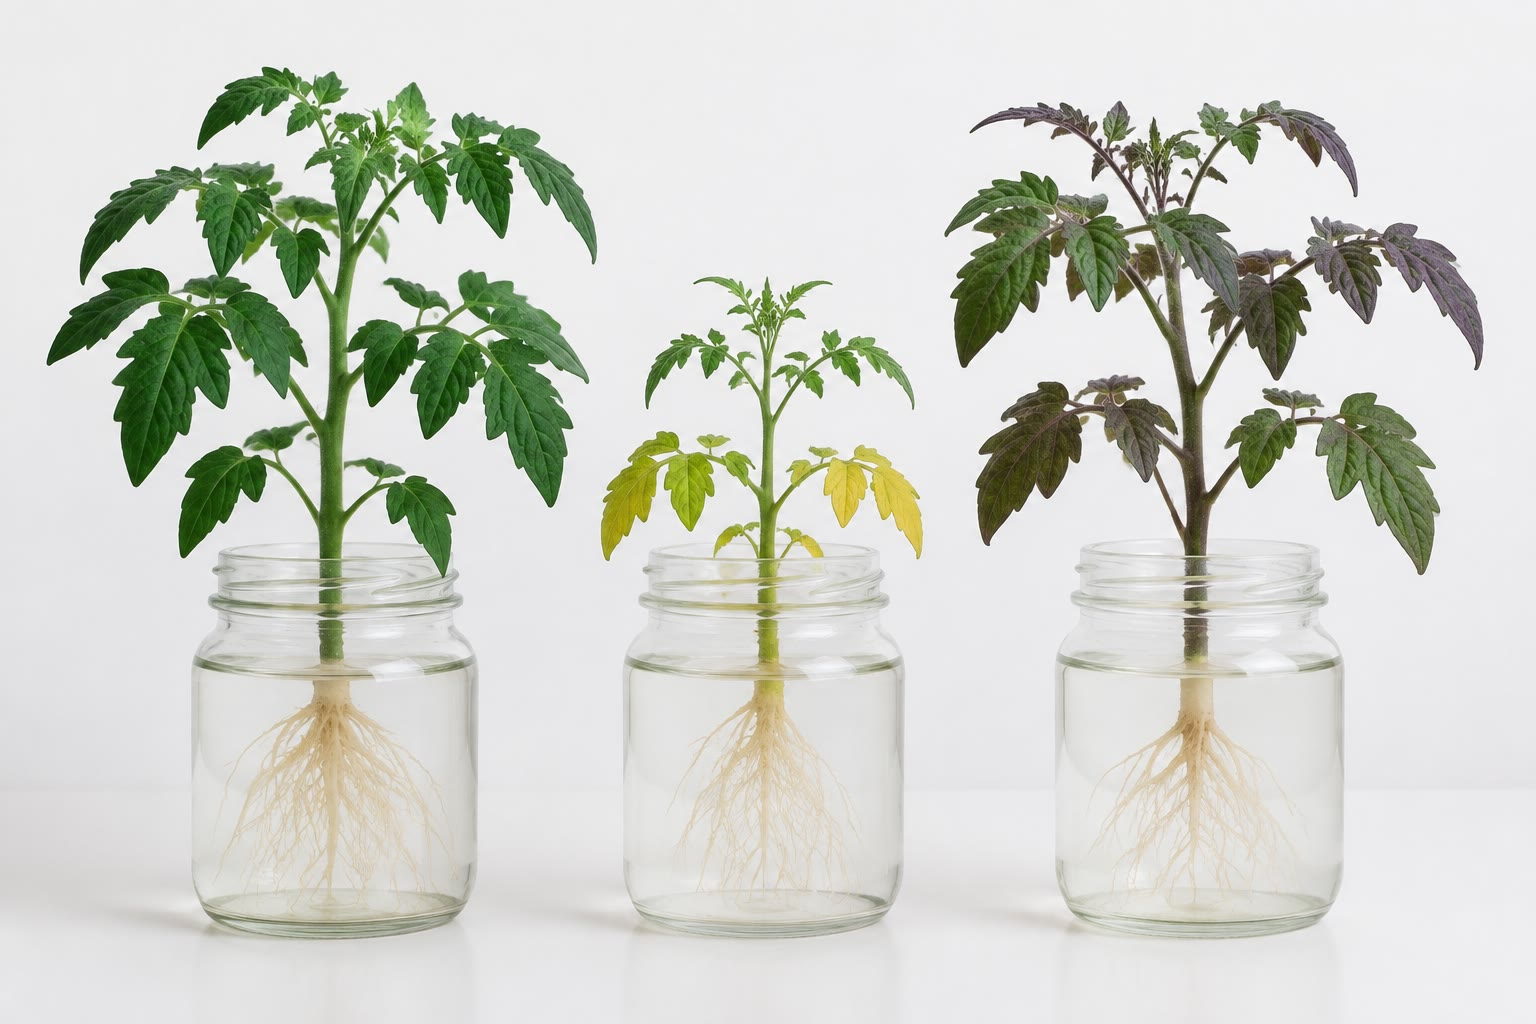
\includegraphics[width=0.6\linewidth]{images/book3/ai/b3-23-nutrient-deficiency.jpg}

{\small 三株番茄植株分别培养于营养液中：完全营养（左）；
缺氮（中：植株矮小，老叶发黄，
因氮已转移至新叶）；缺磷（右：叶色深暗
并带紫色）。每种缺失的元素都有其特征性表现。}
\end{omfigure}

\begin{method}[读取缺素症状]\label{met:b1:plant-water-minerals:deficiency}
\begin{enumerate}
  \item 观察症状出现在何处。植物可经\omterm{def:b1:flowering-plant-organization:tissues}{韧皮部}转运的元素
        （N、P、K、Mg）会从老叶中撤回以供给新叶，
        因此老叶最先出现缺素症状。
        植物无法转运的元素（Ca、Fe、B）则留在最初沉积之处，
        故幼叶与生长点率先表现出症状。
  \item 思考该元素的作用：缺氮，\omterm{def:b1:photosynthesis:pigments}{叶绿素}与\omterm{def:b1:proteins:peptide}{蛋白质}减少，
        叶色苍白、植株矮小；缺镁或缺铁，\omterm{def:b1:photosynthesis:pigments}{叶绿素}失效，
        叶片发黄而叶脉仍为绿色；缺钾，
        叶缘焦枯；缺钙，生长点枯死。
  \item 单独供给所怀疑的元素，
        并观察新生长的部分，以此确认。
\end{enumerate}
\end{method}

\begin{proposition}[离子的主动吸收]\label{prop:b1:plant-water-minerals:uptake}
\index{质子泵}
土壤溶液中离子的浓度为微摩尔至几毫摩尔每
升；根\omterm{def:b1:cell-unit-of-life:cell}{细胞}中钾的浓度为 \qty{100}{mmol/L}，磷酸盐
为 \qty{10}{}，硝酸盐则为若干。因此吸收多为逆浓度进行，
需消耗 \omterm{def:b1:water-small-molecules:atp}{ATP}，但方式较为间接：\omterm{def:b1:membranes-transport:membrane}{质膜}中的\emph{\omterm{prop:b1:plant-water-minerals:uptake}{质子泵}}
（\cref{ch:b1:membranes-transport}）向外排出 $\mathrm{H^+}$，
使膜外呈酸性，膜内电位达
\qtyrange{-120}{-200}{mV}；阳离子如 $\mathrm{K^+}$ 顺电场梯度经通道进入，
阴离子
（$\mathrm{NO_3^-}$、$\mathrm{H_2PO_4^-}$、$\mathrm{SO_4^{2-}}$）则借
\omterm{prop:b1:membranes-transport:secondary}{同向转运体}与质子一同回流而被运入。转运蛋白具有选择性：
钾的吸收比与其电荷相同、大小
相近的钠快百倍，植物即便在盐渍土中
也能将钠拒于体外。根系将植物三分之一的呼吸作用
用于这一运输。
\end{proposition}

\section{氮}

\begin{proposition}[硝酸盐转化为氨基酸]\label{prop:b1:plant-water-minerals:nitrate}
\index{硝酸还原酶}\index{氮同化}
多数植物以硝酸盐的形式吸收氮。在\omterm{def:b1:eukaryotic-cell:organelle}{细胞溶胶}中，\emph{\omterm{prop:b1:plant-water-minerals:nitrate}{硝酸还原酶}}
是一种含钼的酶，借 NADH 提供的电子将其还原为亚硝酸盐；
在\omterm{def:b1:eukaryotic-cell:plastid}{质体}中，\emph{亚\omterm{prop:b1:plant-water-minerals:nitrate}{硝酸还原酶}}借铁氧还蛋白提供的电子
将亚硝酸盐还原为铵；铵随即固定为
谷氨酰胺和\omterm{def:b1:biosyntheses-integration:nitrogen}{谷氨酸}（\cref{ch:b1:biosyntheses-integration}）
——铵本身有毒，从不积累。整个还原过程
每个氮耗八个电子，约占富含硝酸盐土壤中叶片
光合电子流的十分之一，叶片大部分还原
在光下完成，直接取自\omterm{def:b1:photosynthesis:chloroplast}{叶绿体}的铁氧还蛋白。土壤中若有铵，
植物可直接吸收，无需付出此代价。
\end{proposition}

\begin{definition}[固氮与根瘤]\label{def:b1:plant-water-minerals:nodules}
\index{固氮}\index{根瘤}\index{Rhizobium}
没有真核生物能利用空气中的 $\mathrm{N_2}$。部分细菌能够：
\emph{固氮酶}断开 $\mathrm{N_2}$ 的三键，
并将其还原为两分子氨，每分子耗十六个 \omterm{def:b1:water-small-molecules:atp}{ATP} 与八个电子，
且仅在隔绝氧气处进行。豆科植物（豌豆、菜豆、三叶草）
将这类细菌（\emph{Rhizobium}）容纳于
\emph{根瘤}之中：植物构造出一个腔室，为细菌供给糖分，
并借红色的豆血红蛋白维持低氧，
它将氧输送至细菌的呼吸作用，浓度低至不致伤害酶；
细菌则回馈铵，植物将其转化为\omterm{def:b1:proteins:aminoacid}{氨基酸}。一块三叶草田
每年每公顷可固定约一百千克氮，植物为此付出其光合作用的
十分之一。整个氮循环
的全部内容
属于本科二年级分册。
\end{definition}

\begin{omfigure}
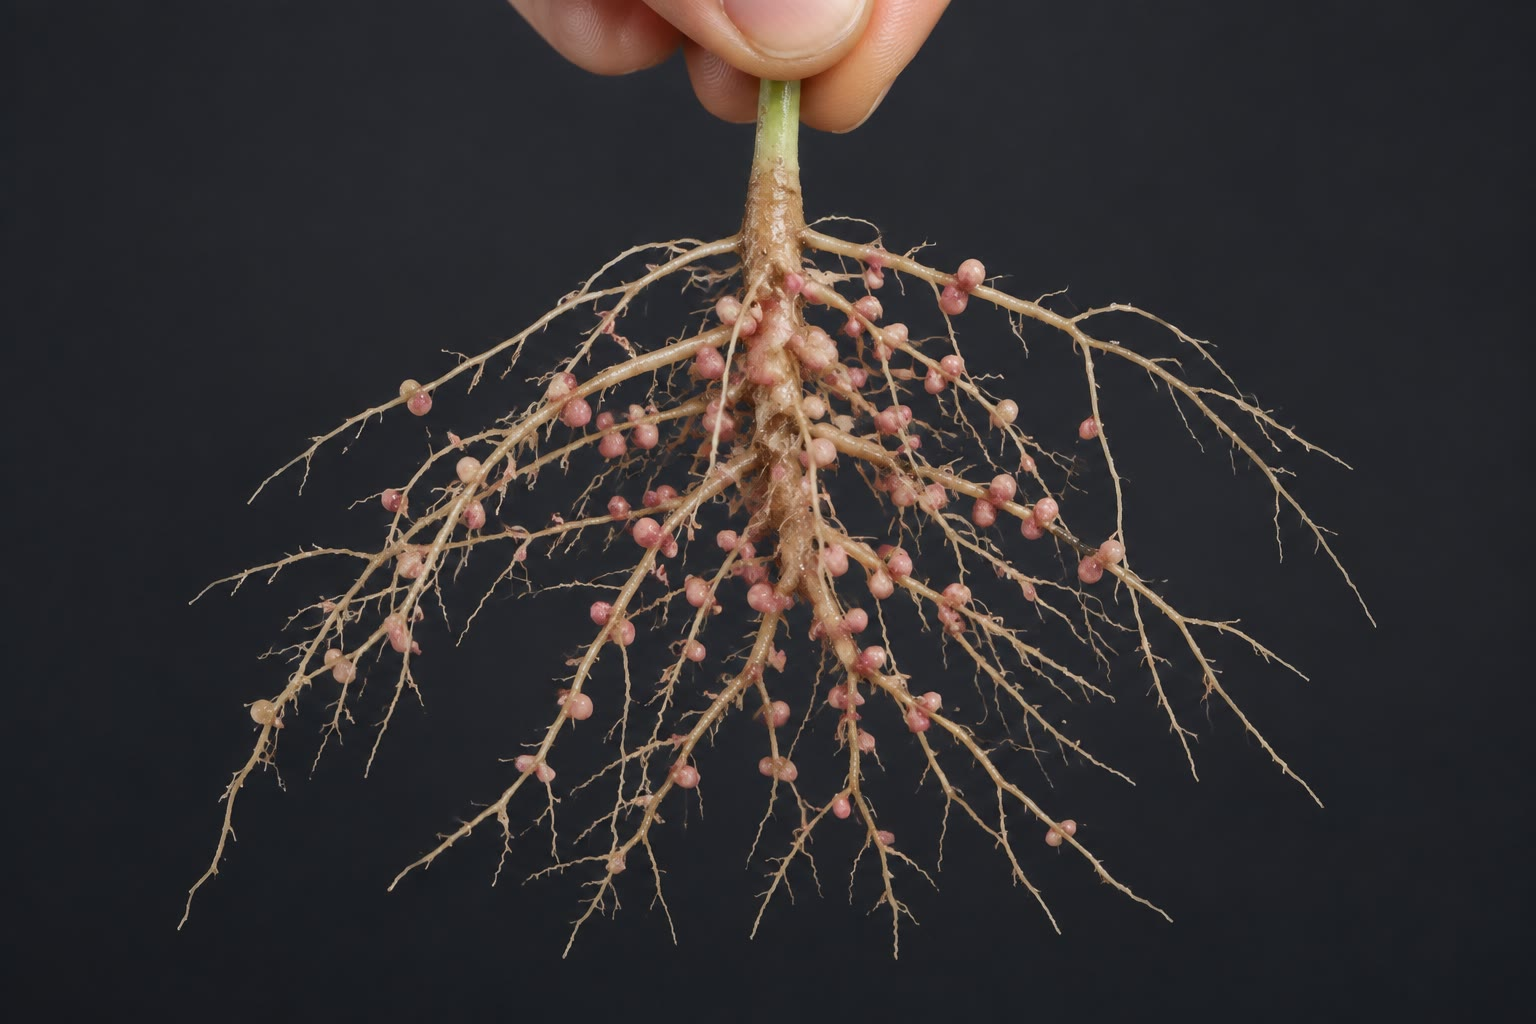
\includegraphics[width=0.52\linewidth]{images/book3/ai/b3-23-root-nodules.jpg}

{\small 豆科植物根上的\omterm{def:b1:plant-water-minerals:nodules}{根瘤}：每个\omterm{def:b1:plant-water-minerals:nodules}{根瘤}都是充满细菌的植物\omterm{def:b1:body-plans-tissues:tissue}{组织}腔室，
其中充满细菌，因含豆血红蛋白而呈粉红色，大气中的氮
在此被固定。}
\end{omfigure}

\begin{example}[氮的代价]\label{ex:b1:plant-water-minerals:priceN}
一株玉米每天约需 \qty{30}{mg} 氮，取自
浓度为 \qty{2}{mmol/L} 的硝酸盐溶液，它每蒸腾一升水便获得这些氮，
并耗费数百毫摩尔电子将其还原。
若由三叶草固定同样数量的氮，每个
$\mathrm{N_2}$ 需 \qty{16}{} 个 \omterm{def:b1:water-small-molecules:atp}{ATP}，外加还原剂——约合 \qty{6}{g} 糖
每克氮，每天约 \qty{0.2}{g}，占其产量的十分之一
——且可在完全没有硝酸盐的土壤中生长。农民
两千年来一直将豆科植物与谷类轮作，以便把这些氮
从一块田转移到下一块田。
\end{example}

\section{土壤中的伙伴}

\begin{definition}[菌根]\label{def:b1:plant-water-minerals:mycorrhiza}
\index{菌根}
\emph{菌根}是根与真菌之间的一种共生关系，
见于十分之九的植物中。最常见的形式中，真菌的
菌丝伸入皮层\omterm{def:b1:cell-unit-of-life:cell}{细胞}，并在\omterm{def:b1:cell-unit-of-life:cell}{细胞}内分支形成
\emph{丛枝}，即交换表面；而在根外，
一张直径仅数微米的菌丝网在土壤中探索，范围可达
数米。真菌向植物输送磷酸盐及其他移动性差的离子，
以及\omterm{def:b1:flowering-plant-organization:organs}{根毛}自身无法触及的水分；植物则
向真菌输送糖分，约占其光合作用的十分之一或更多。温带森林的树木
还具有第二种形式：真菌包裹
根尖并在\omterm{def:b1:cell-unit-of-life:cell}{细胞}之间穿行；其子实体
即林地上的蘑菇。
\end{definition}
\begin{proof}[证据]
在灭菌土壤中生长的幼苗长势不良，吸收的
磷酸盐也很少；接种该真菌孢子后，幼苗长得
大数倍。放射性磷酸盐施于根系所不能及的
土壤中，只有当菌丝将两者相连时才会出现在植物体内，
而饲喂叶片的标记碳一天之内即出现在菌丝中。
以细网将菌丝隔开，网眼允许溶质通过而不允许真菌通过，
这一增益便随之消失。
\end{proof}

\begin{omfigure}
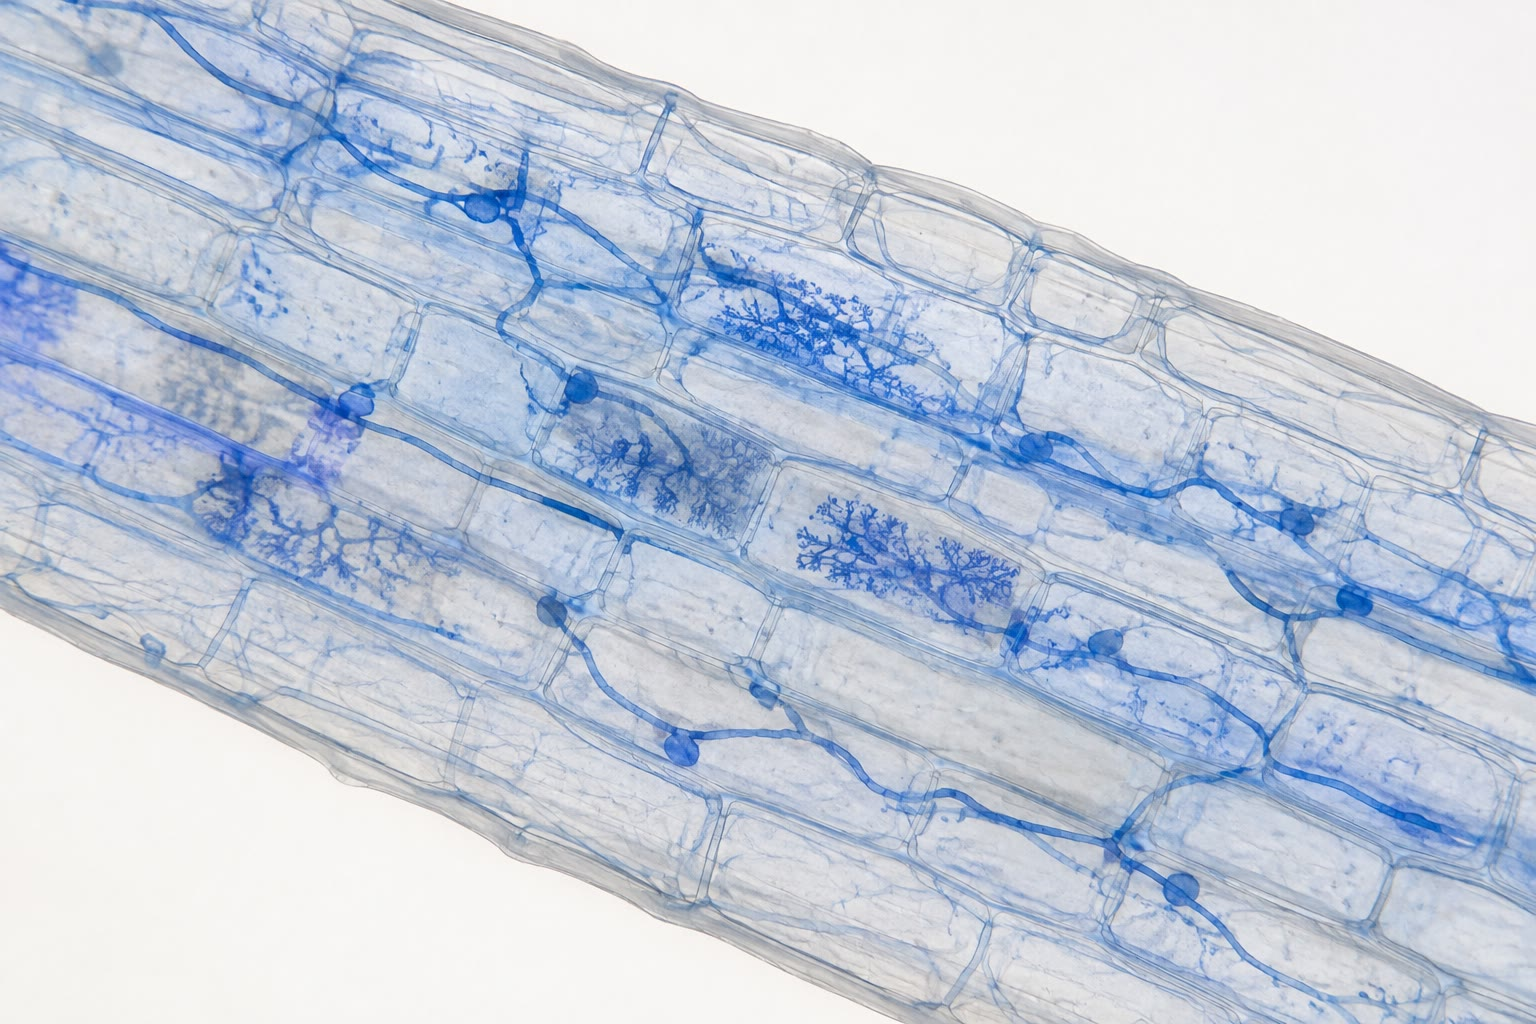
\includegraphics[width=0.52\linewidth]{images/book3/ai/b3-23-mycorrhiza.jpg}

{\small 经染色以显示\omterm{def:b1:plant-water-minerals:mycorrhiza}{菌根}真菌的根：菌丝
在\omterm{def:b1:cell-unit-of-life:cell}{细胞}间穿行，并在\omterm{def:b1:cell-unit-of-life:cell}{细胞}内分支形成丛枝——这是
第二个吸收面，由植物以糖分供养。}
\end{omfigure}

\begin{example}[为何磷酸盐需要真菌]\label{ex:b1:plant-water-minerals:phosphate}
磷酸盐与土壤颗粒结合，一天内仅扩散约一毫米；
\omterm{def:b1:flowering-plant-organization:organs}{根毛}在数小时内即吸尽可及范围内的全部磷酸盐，随后
便只能等待。直径为\omterm{def:b1:flowering-plant-organization:organs}{根毛}十分之一的菌丝，单位\omterm{def:b1:body-plans-tissues:tissue}{组织}量下
可延伸至十倍远，且一米菌丝对植物而言的成本
仅为一米根所耗成本的千分之一。对于随土壤水分自由移动的硝酸盐，
\omterm{def:b1:flowering-plant-organization:organs}{根毛}本身即已足够，富含硝酸盐的土壤上的植物
会减少与真菌的共生；而对于磷酸盐，真菌即是根的
延伸部分。
\end{example}

\section{练习}

\begin{exercise}[$\star$]\label{exo:b1:plant-water-minerals:1}
定义\omterm{def:b1:plant-water-minerals:pathways}{质外体}和\omterm{def:b1:plant-water-minerals:pathways}{共质体}，并说明\omterm{def:b1:plant-water-minerals:pathways}{凯氏带}的作用。
\end{exercise}

\begin{exercise}[$\star$]\label{exo:b1:plant-water-minerals:2}
列出植物从土壤中吸收的六种\omterm{def:b1:plant-water-minerals:elements}{大量元素}，
并说明每种元素的一种作用。
\end{exercise}

\begin{exercise}[$\star$]\label{exo:b1:plant-water-minerals:3}
由\omterm{def:b1:membranes-transport:osmosis}{水势}图读出土壤、根\omterm{def:b1:flowering-plant-organization:tissues}{木质部}和叶\omterm{def:b1:cell-unit-of-life:cell}{细胞}中的 $\Psi$，
并说明每一步的水流方向。
\end{exercise}

\begin{exercise}[$\star$]\label{exo:b1:plant-water-minerals:4}
为什么缺氮和缺铁的症状会出现在不同的
叶片上？
\end{exercise}

\begin{exercise}[$\star\star$]\label{exo:b1:plant-water-minerals:5}
一个根皮层\omterm{def:b1:cell-unit-of-life:cell}{细胞}的 $\Psi_s = \qty{-0.9}{MPa}$，且 $\Psi_p =
\qty{0.5}{MPa}$；土壤\omterm{def:b1:membranes-transport:osmosis}{水势}为 \qty{-0.2}{MPa}，\omterm{def:b1:flowering-plant-organization:tissues}{木质部}为
\qty{-0.6}{MPa}。证明水分由土壤经\omterm{def:b1:cell-unit-of-life:cell}{细胞}流入\omterm{def:b1:flowering-plant-organization:tissues}{木质部}，并计算该\omterm{def:b1:cell-unit-of-life:cell}{细胞}
恰好停止从此土壤吸水时的
$\Psi_p$。
\end{exercise}

\begin{exercise}[$\star\star$]\label{exo:b1:plant-water-minerals:6}
计算相对湿度为 \qty{90}{\%}、\qty{50}{\%} 和
\qty{10}{\%} 时、\qty{25}{\celsius} 下空气的\omterm{def:b1:membranes-transport:osmosis}{水势}（$RT/V_w =
\qty{137}{MPa}$）。与萎蔫点的土壤\omterm{def:b1:membranes-transport:osmosis}{水势}相比，
并加以评论。
\end{exercise}

\begin{exercise}[$\star\star$]\label{exo:b1:plant-water-minerals:7}
\omterm{def:b1:membranes-transport:potential}{膜电位}为 \qty{-150}{mV} 的根\omterm{def:b1:cell-unit-of-life:cell}{细胞}吸收 $\mathrm{K^+}$，
使其浓度由 \qty{0.1}{mmol/L} 升至 \qty{100}{mmol/L}。计算该浓度比在 \qty{25}{\celsius} 下的
能斯特电位，并判断单靠通道能否完成这一过程。
对硝酸根重复上述计算，外部为 \qty{0.5}{}
、内部为 \qty{5}{mmol/L}。
\end{exercise}

\begin{exercise}[$\star\star$]\label{exo:b1:plant-water-minerals:8}
解释为何吐水现象在草上于黎明时可见，而在高大的树上从不出现，
并说明蒸腾作用开始后\omterm{prop:b1:plant-water-minerals:rootpressure}{根压}会发生什么变化。
\end{exercise}

\begin{exercise}[$\star\star$]\label{exo:b1:plant-water-minerals:9}
将一株植物转入缺钼的溶液。预测其
分别以硝酸盐和铵盐为氮源时的生长状况，并解释二者的差异。
\end{exercise}

\begin{exercise}[$\star\star\star$]\label{exo:b1:plant-water-minerals:10}
计算每天将 \qty{30}{mg} 硝态氮还原为铵所需的电子数，
以及所需的 \omterm{def:b1:biosyntheses-integration:ppp}{NADPH} 当量数，并与
一片面积为 \qty{500}{cm^2} 的玉米叶在一天内经\omterm{def:b1:photosynthesis:zscheme}{光系统}
传递的电子数相比较，取固定速率为每平方米每秒 \qty{4}{\micro mol} $\mathrm{CO_2}$，
（每个 $\mathrm{CO_2}$ 对应 4 个电子，光照 \qty{12}{h}）。
\end{exercise}

\begin{exercise}[$\star\star\star$]\label{exo:b1:plant-water-minerals:11}
一株三叶草每天固定 \qty{30}{mg} 氮，固定每个 $\mathrm{N_2}$ 需
消耗 \qty{16}{} 个 \omterm{def:b1:water-small-molecules:atp}{ATP} 和 \qty{8}{} 个电子，总体上每克氮需
消耗 \qty{6}{g} 糖。计算\omterm{def:b1:plant-water-minerals:nodules}{固氮}酶单独消耗的 \omterm{def:b1:water-small-molecules:atp}{ATP} 量、
按每个葡萄糖可产生 30 个 \omterm{def:b1:water-small-molecules:atp}{ATP} 计算所需的糖量，以及这部分占
\qty{6}{g} 的比例。其余的糖用于何处？
\end{exercise}

\begin{exercise}[$\star\star\star$]\label{exo:b1:plant-water-minerals:12}
“根是一座雇用承包商的采矿作业。”请用一段话讨论：根自身做什么
（水分、可移动离子），外包什么（磷酸盐、固定氮），
付出什么代价，
以及何时停止付出代价。
\end{exercise}

\section{问题：玉米根的水势阶梯}

\begin{problem}[{周末问题——七月土壤中的水分与硝酸盐进入玉米植株：
各步的水势，经根的通量，
所携带的氮及还原它的代价，
最后落在进入根部的每日水通量上}]
\label{pb:b1:plant-water-minerals:1}
一株七月的玉米：细根表面积 \qty{0.2}{m^2}，根的水力
导度为 \qty{2e-7}{m.s^{-1}.MPa^{-1}}；叶面积
为 \qty{0.5}{m^2}。土壤\omterm{def:b1:membranes-transport:osmosis}{水势}为 \qty{-0.2}{MPa}；根皮层\omterm{def:b1:cell-unit-of-life:cell}{细胞}
的 $\Psi_s = \qty{-0.9}{MPa}$，$\Psi_p = \qty{0.5}{MPa}$；根\omterm{def:b1:flowering-plant-organization:tissues}{木质部}
为 \qty{-0.6}{MPa}；叶\omterm{def:b1:cell-unit-of-life:cell}{细胞}为 \qty{-1.3}{MPa}；空气
相对湿度为 \qty{50}{\%}（$RT/V_w = \qty{137}{MPa}$）。土壤硝酸盐
浓度为 \qty{2}{mmol/L}；该植株每天需要 \qty{30}{mg} 氮。
硝酸盐还原为铵时每个氮消耗 8 个电子；
光合作用每固定一个 $\mathrm{CO_2}$ 传递 4 个电子，叶片
每平方米每秒固定 \qty{4}{\micro mol} 的 $\mathrm{CO_2}$，持续
\qty{12}{h}。

\medskip
\noindent\textbf{第一部分——\omterm{def:b1:membranes-transport:osmosis}{水势}阶梯。}
\begin{enumerate}
  \item 计算根皮层\omterm{def:b1:cell-unit-of-life:cell}{细胞}的\omterm{def:b1:membranes-transport:osmosis}{水势}。
  \item 写出土壤、皮层、\omterm{def:b1:flowering-plant-organization:tissues}{木质部}、叶的顺序，并验证
        每一步水流都向内、向上流动。
  \item 计算空气的\omterm{def:b1:membranes-transport:osmosis}{水势}。
  \item 计算从土壤到叶的降幅，以及从叶到空气的降幅；
        最后一步占总降幅的比例是多少？
  \item 土壤干燥至 \qty{-0.9}{MPa}。进入皮层\omterm{def:b1:cell-unit-of-life:cell}{细胞}的水流
        及其\omterm{def:b1:eukaryotic-cell:plantcell}{膨压}会发生什么变化？
  \item 土壤干燥至 \qty{-1.5}{MPa}。叶片会发生什么变化，
        为何浇水能使其恢复？
\end{enumerate}

\medskip
\noindent\textbf{第二部分——通量。}
\begin{enumerate}[resume]
  \item 计算流入根的水流通量（电导 $\times$
        表面积 $\times$ 土壤与根\omterm{def:b1:flowering-plant-organization:tissues}{木质部}之间的差值）。
  \item 将其换算为每天的升数。
  \item 这些水全部通过蒸腾作用散失，
        计算每平方米叶片每小时的蒸腾量，以克为单位。
  \item 将每平方米叶片每秒的蒸腾量换算为
        毫摩尔水（\qty{18}{g/mol}）。
  \item 正午时\omterm{def:b1:flowering-plant-organization:tissues}{气孔}关闭，叶片的 $\Psi$ 升至
        \qty{-0.9}{MPa}，\omterm{def:b1:flowering-plant-organization:tissues}{木质部}的\omterm{def:b1:membranes-transport:osmosis}{水势}升至 \qty{-0.4}{MPa}。
        重新计算通量。植物做了什么？为什么？
  \item 为什么根吸收水分无需消耗能量，
        而吸收硝酸盐却必须消耗能量？
\end{enumerate}

\medskip
\noindent\textbf{第三部分——氮。}
\begin{enumerate}[resume]
  \item 计算第 8 题中水流通量带入根的硝酸盐量，
        分别以毫摩尔和毫克氮为单位。
  \item 它能否满足植物的需求？平衡会发生什么变化？
  \item 根在其\omterm{def:b1:cell-unit-of-life:cell}{细胞}内将硝酸盐积累至 \qty{5}{mmol/L}。
        计算一摩尔物质从外部
        \qty{2}{mmol/L} 移入内部 \qty{5}{mmol/L} 所需的\omterm{prop:b1:water-small-molecules:gibbs}{自由能}，
        在\omterm{def:b1:membranes-transport:potential}{膜电位}为 \qty{-150}{mV} 的情况下（$RT = \qty{2.48}{kJ/mol}$；
        阴离子进入带负电的\omterm{def:b1:cell-unit-of-life:cell}{细胞}）。
  \item 该吸收过程是与两个质子的同向转运。计算两个质子
        在 \qty{-150}{mV} \omterm{def:b1:membranes-transport:potential}{膜电位}下进入\omterm{def:b1:cell-unit-of-life:cell}{细胞}时释放的\omterm{prop:b1:water-small-molecules:gibbs}{自由能}，
        即从 \omterm{def:b1:water-small-molecules:ph}{pH} 5.5 到 \omterm{def:b1:water-small-molecules:ph}{pH} 7.5，并检验其是否足够。
  \item 计算每天将
        \qty{30}{mg} 氮还原为铵所需的电子数。
  \item 计算叶片每天通过其\omterm{def:b1:photosynthesis:zscheme}{光系统}传递的电子数，
        以及转向硝酸盐的电子比例。
\end{enumerate}

\medskip
\noindent\textbf{第四部分——其他情形。}
\begin{enumerate}[resume]
  \item 若土壤提供铵而非硝酸盐，植物会节省什么，
        而铵的吸收会给
        其 \omterm{def:b1:water-small-molecules:ph}{pH} 平衡带来什么问题？
  \item 三叶草每天固定同样的 \qty{30}{mg} 氮，
        若每个 $\mathrm{N_2}$ 耗用 \qty{16}{} 个 \omterm{def:b1:water-small-molecules:atp}{ATP} 和 \qty{8}{} 个电子，
        计算\omterm{def:b1:plant-water-minerals:nodules}{固氮}酶每天消耗的 \omterm{def:b1:water-small-molecules:atp}{ATP}。
  \item 每固定一克氮（总计）需消耗 \qty{6}{g} 糖，
        计算三叶草每天的糖耗，并与
        每天 \qty{3}{g} 糖的产量相比较。这笔交易
        在硝酸盐浓度为 \qty{2}{mmol/L} 的土壤中是否划算？
        在不含硝酸盐的土壤中呢？
  \item 土壤溶液中磷酸盐的浓度为 \qty{2}{\micro mol/L}。
        计算第 8 题中水流带入的磷酸盐量，
        并与植物每天 \qty{4}{mg} 磷的需求
        （\qty{31}{g/mol}）相比较。植物必须依赖什么？
  \item 用两句话说明\omterm{def:b1:plant-water-minerals:pathways}{凯氏带}如何使根
        在\omterm{def:b1:flowering-plant-organization:tissues}{木质部}中保持 \qty{5}{mmol/L} 的硝酸盐，
        而土壤中的值为 \qty{2}{}。
  \item 一株突变体缺乏\omterm{def:b1:plant-water-minerals:pathways}{凯氏带}，预测其\omterm{def:b1:flowering-plant-organization:tissues}{木质部}汁液的组成，
        以及它在盐渍土壤中的表现。
  \item 陈述结果：玉米根每天的水流通量，
        其输送的氮量，以及叶片电子中
        用于将其还原的比例。
\end{enumerate}
\end{problem}
